Ce chapitre traite des aspects DevOps et MLOps mis en place durant la réalisation du projet, dans le but d'automatiser au maximum les tâches opérationnelles. Ces aspects comprennent notamment la mise en place de pipelines de déploiement automatiques du code, ainsi que de pipelines d'entraînement et d'évaluation automatiques de modèles de machine-learning.

\section{DevOps}
Le DevOps est un "ensemble de pratiques qui met l’accent sur la collaboration et la communication entre les développeurs de logiciels et les professionnels des opérations informatiques, en automatisant le processus de livraison de logiciel et les changements d’infrastructure" \cite{devops}.

Dans le cadre de ce projet l'aspect DevOps principal est la mise en place d'un processus automatisé pour déployer efficacement la chaîne de services développés.

\subsection{Structure du Git}
La solution choisie pour héberger le code est le mono-repo. C'est à dire que le code des différents services que composent le workflow sont tous sur le même repository Git, dans un dossier \verb|code|. La plate-forme choisie est GitHub. La figure \ref{fig:repo} montre comment est organisée le dossier \verb|code| du repository.

\begin{figure}[H]
    \centering
    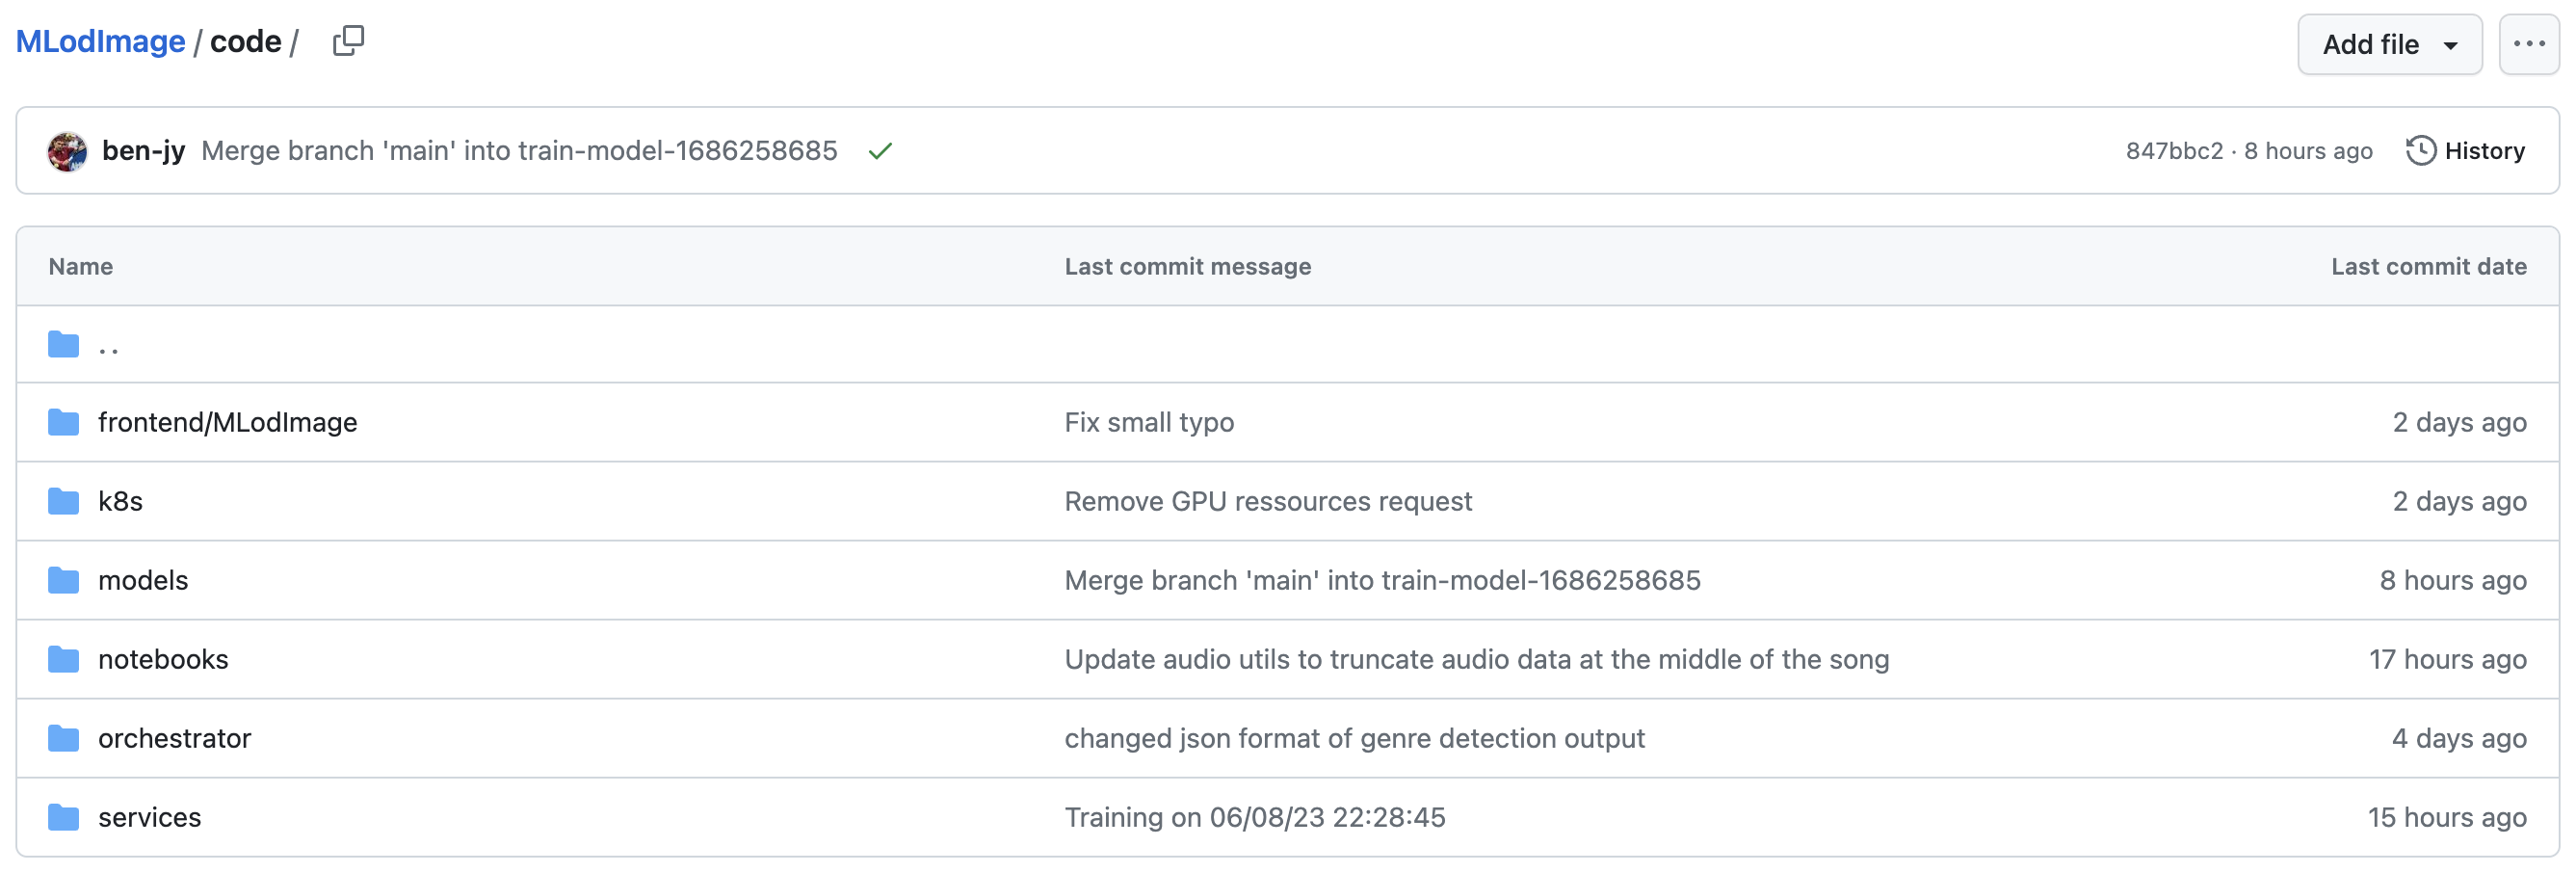
\includegraphics[width=1\textwidth]{rapport_PI/rsc/struct_repo.png}
    \caption{Structure du dossier code du repository Git.}
    \label{fig:repo}
\end{figure}

\subsection{Infrastructure de déploiement}
Pour faire tourner notre chaîne de services, un cluster Kubernetes est mis à disposition. De ce fait, chaque service doit avoir une Dockerfile, afin de pouvoir construire l'image d'un container dans lequel il va tourner. Ces images seront ensuite stockées sur la container-registry intégrée à GitHub, pour être exécutées sur le cluster.

\subsection{Approche choisie}
Afin de simplifier au maximum le déploiement des différents services pour tout le monde, l'approche choisie est d'avoir une seule pipeline de déploiement, qui va s'occuper de détecter les différents services et de les déployer, sans que les développeurs aient à écrire leur propre Github Workflow. Les différents services ont donc été généralisés (Des instruction ont été données pour l'écriture de la Dockerfile, notamment le port qui va être routé vers l'endpoint du service). Afin que les développeurs puissent quand même personnaliser un peu l'infrastructure sur laquelle va tourner leur service, des fichier "flags" ont été introduits. C'est-à-dire que dans le dossier du service en question, le développeur peut introduire une fichier qui correspond à un des deux flags disponibles :

\begin{itemize}
    \item \verb|.gpu| :  Fichier pour demander à ce que le service soit déployé sur un noeud qui contient un GPU. En plus de ce fichier, il doit y inscrire une valeur entière, qui est la quantité de mémoire vidéo souhaitée, en tranche de 256Mb \cite{k8s_gpu}.
    \item \verb|.build-only| :  Fichier afin que l'image Docker du service soit construite et publiée sur la registry, mais pas déployée sur le cluster.
\end{itemize}

En plus de ces flags, les développeurs ont également la possibilité d'écrire une script shell qui sera exécuté \textbf{avant} la construction de l'image Docker. Pour cela, il faut que ce script aie comme nom de fichier \verb|pre.sh|.

Avec cette approche, les développeurs n'ont presque rien à faire, si ce n'est d'adapter une Dockerfile type pour leur services en y ajoutant les potentiels installations hors dépendances Python.


\subsection{Pipeline de déploiement}
La pipeline de déploiement se déclenche à chaque push sur la branche main. Dans un premier temps, l'instance du runner qui exécute la pipeline va s'assurer d'avoir les accès nécessaire au cluster et a la registry, et aussi que les variables d'environnement nécessaires aux Pods sont bien créées sur le cluster. Finalement, vient la partie déploiement automatique. Pour se faire, un script Python est utilisé pour détecter les services à (re)déployer. Voici les étapes présentent dans ce script: 

\begin{itemize}
    \item \textbf{Détection des changements : }Afin d'éviter de redéployer tout le code du repository à chaque micro-modification d'un service, un mécanisme de détection des changement est en place grâce à la commande \verb|git diff|. En comparant l'avant dernier commit avec le dernier, on obtient une liste de fichiers modifié, on peut alors en déduire quels service il faut redéployer. Petit bémol, si l'on push plusieurs commits à la fois, il est possible que des changements ne soient pas détectés, du au fait que l'on compare uniquement les deux derniers commit.
    \item \textbf{Détection des services à déployer : } La deuxième étape est de parcourir le dossier services, si dans ce dernier se trouve un sous-dossier contenant une Dockerfile, le script considère que c'est un service à déployer. Si le service (dont le nom correspond au nom du dossier qui le contiens) est détecté comme ayant subi un changement, le script va effectuer les étapes qui suivent sur le service en question.
    \item \textbf{Build et publication des images Docker : } Cette étape consiste à construire l'image décrite par la Dockerfile, puis de la publier sur la registry du projet. Mais avant, si un script pré-build est présent dans le service, ce dernier sera exécuté.
    \item \textbf{Déploiement du service sur le cluster : }C'est la dernière étape. Cette étape consiste à regarder si des flags sont présents afin d'adapter le déploiement. Puis, le script va appliquer un fichier yaml qui contient toutes les directives pour déployer un service sur Kubernetes. Afin que cela soit possible, l'outil envsubst est utilisé pour substituer des variables d'environnement dans un fichier, ce qui permet de n'avoir qu'un seul fichier source qui sera ajusté en fonction du nom et des flags du service. Chaque service déployé a alors son port 8000 qui est accessible sur internet, via le nom de domaine \verb|https://<<nom-service>>-mlodimage.kube.isc.heia-fr.ch|.
\end{itemize}

A noter que les dossiers \verb|frontend| et \verb|orchestrator| sont aussi inspectés par le script de déploiement, comme pour les services, afin d'y effectuer le même traitement.

\section{MLOps}

Le MLOps est un ensemble de bonnes pratiques visant à déployer et maintenir des modèles de machine-learning en production de manière fiable. Plus généralement, il consiste à appliquer les principes du DevOps au domaine du machine-learning. 

Dans ce projet, les pratiques MLOps ne sont appliquées qu'à un seul modèle de machine-learning, à savoir celui responsable de la détection du genre musical d'un fichier audio. Les autres modèles sont des modèles pré-entraînés et ne sont pas fine-tunés, ils ne nécessitent donc pas d'entraînement. Les pratiques MLOps appliquées au modèle sont le versioning des données, le monitoring automatique de l'entraînement, ainsi que l'entraînement et le déploiement automatique du modèle.

\subsection{Versioning des données}

Les données qu'utilisent un modèle changent dans le temps et leur grande taille ne permet généralement pas de les stocker dans un système de versioning comme Git. Pourtant, il est primordial de connaître la version des données utilisées pour entraîner un modèle afin de pouvoir reproduire et comprendre les résultats obtenus.

Dans ce projet, nous utilisons l'outil DVC (\textit{Data Version Control}) \cite{dvc} qui est l'un des outils les plus connus pour versionner les données. Il permet de stocker les données dans un système de stockage externe (S3, Azure, Google Cloud, etc.) et de les versionner dans un dépôt Git. Les dossiers et fichiers trackés par DVC sont remplacés par des liens symboliques (contenant leurs hashs) pointant vers les données stockées dans le système de stockage externe et qui peuvent être versionner par Git. La figure \ref{fig:dvc} illustre le fonctionnement de DVC avec un fichier tracké.

\begin{figure}[H]
    \centering
    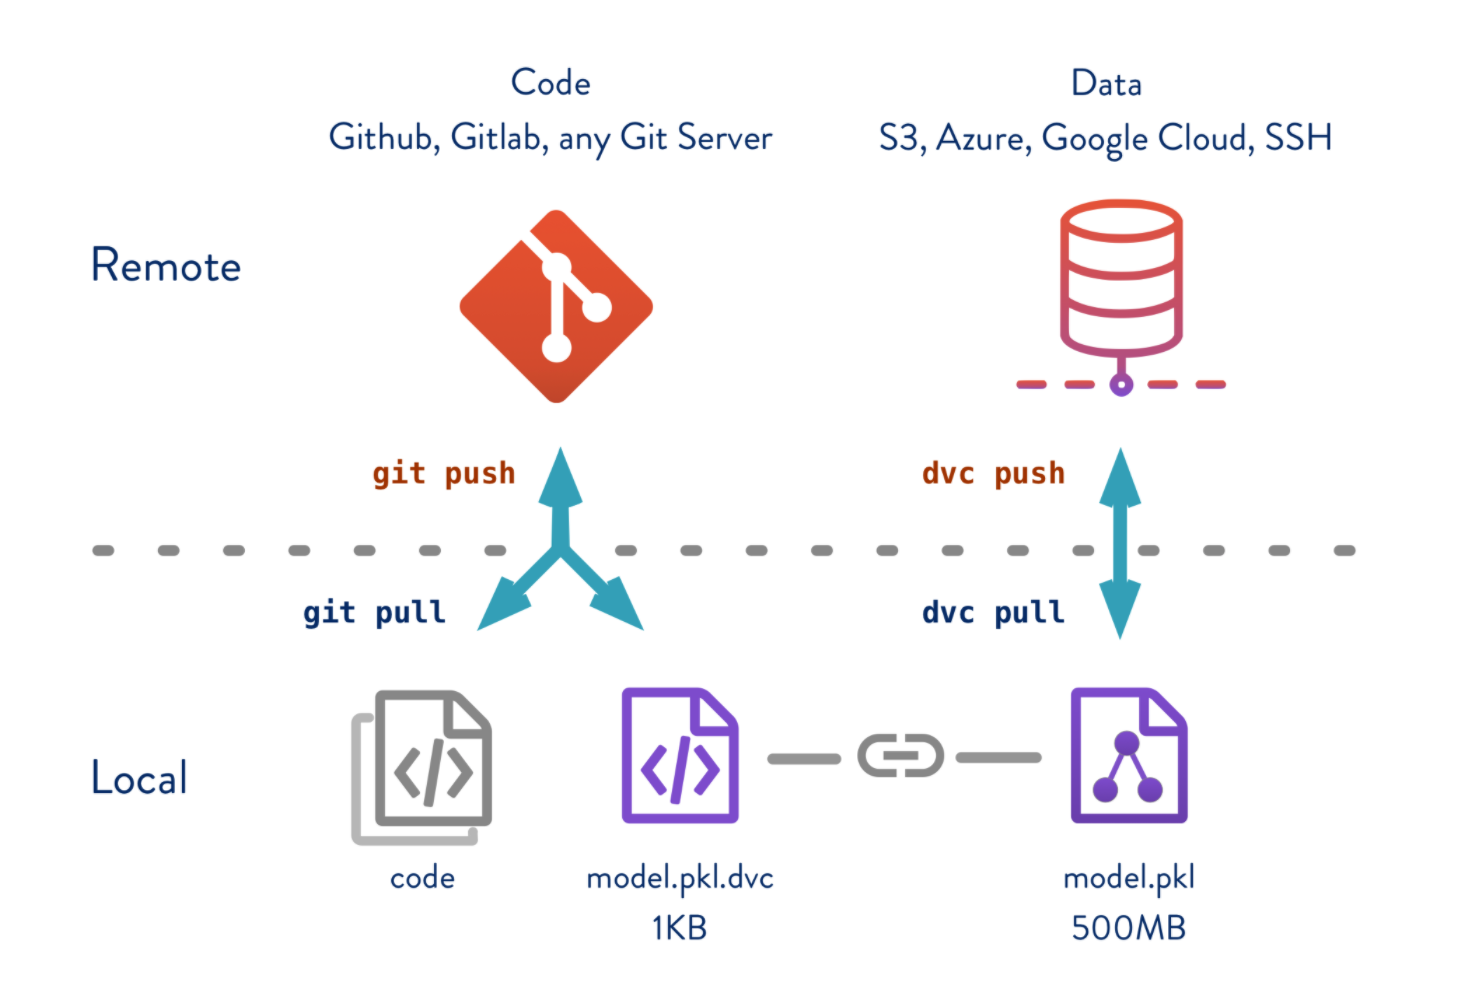
\includegraphics[width=0.7\textwidth]{rsc/git-dvc.png}
    \caption{Fonctionnement de DVC avec un fichier \textit{model.ckpt} tracké.}
    \label{fig:dvc}
\end{figure}

Dans notre cas, nous utilisons le serveur MinIO mis à disposition par l'école comme serveur de stockage, qui est compatible avec l'API S3. DVC permet également de versionner des expériences d'entraînement ainsi que les paramètres, les métriques et les données qui y sont associés. Nous décrivons cet aspect plus en détails dans la section \ref{sec:train_deploy}.

\subsection{Monitoring de l'entraînement}

Il est également important de pouvoir surveiller et suivre l'évolution de l'entraînement d'un modèle afin de pouvoir détecter des comportements indésirables, comme de l'overfitting. Nous utilisons l'outil WandB (\textit{Weight and Biases}) \cite{wandb} pour monitorer l'entraînement de nos modèles. Cet outil permet de visualiser l'évolution du coût, des métriques ou encore des ressources utilisées lors de l'entraînement, simplement en ajoutant quelques lignes de code au script d'entraînement. Cet outil peut également être utilisé pour versionner les données et les modèles entraînés, mais nous avons préféré garder DVC pour cette tâche étant donné que son intégration à Git est plus simple. La figure \ref{fig:wandb} illustre l'interface de WandB après l'entraînement d'un modèle.

\begin{figure}[H]
    \centering
    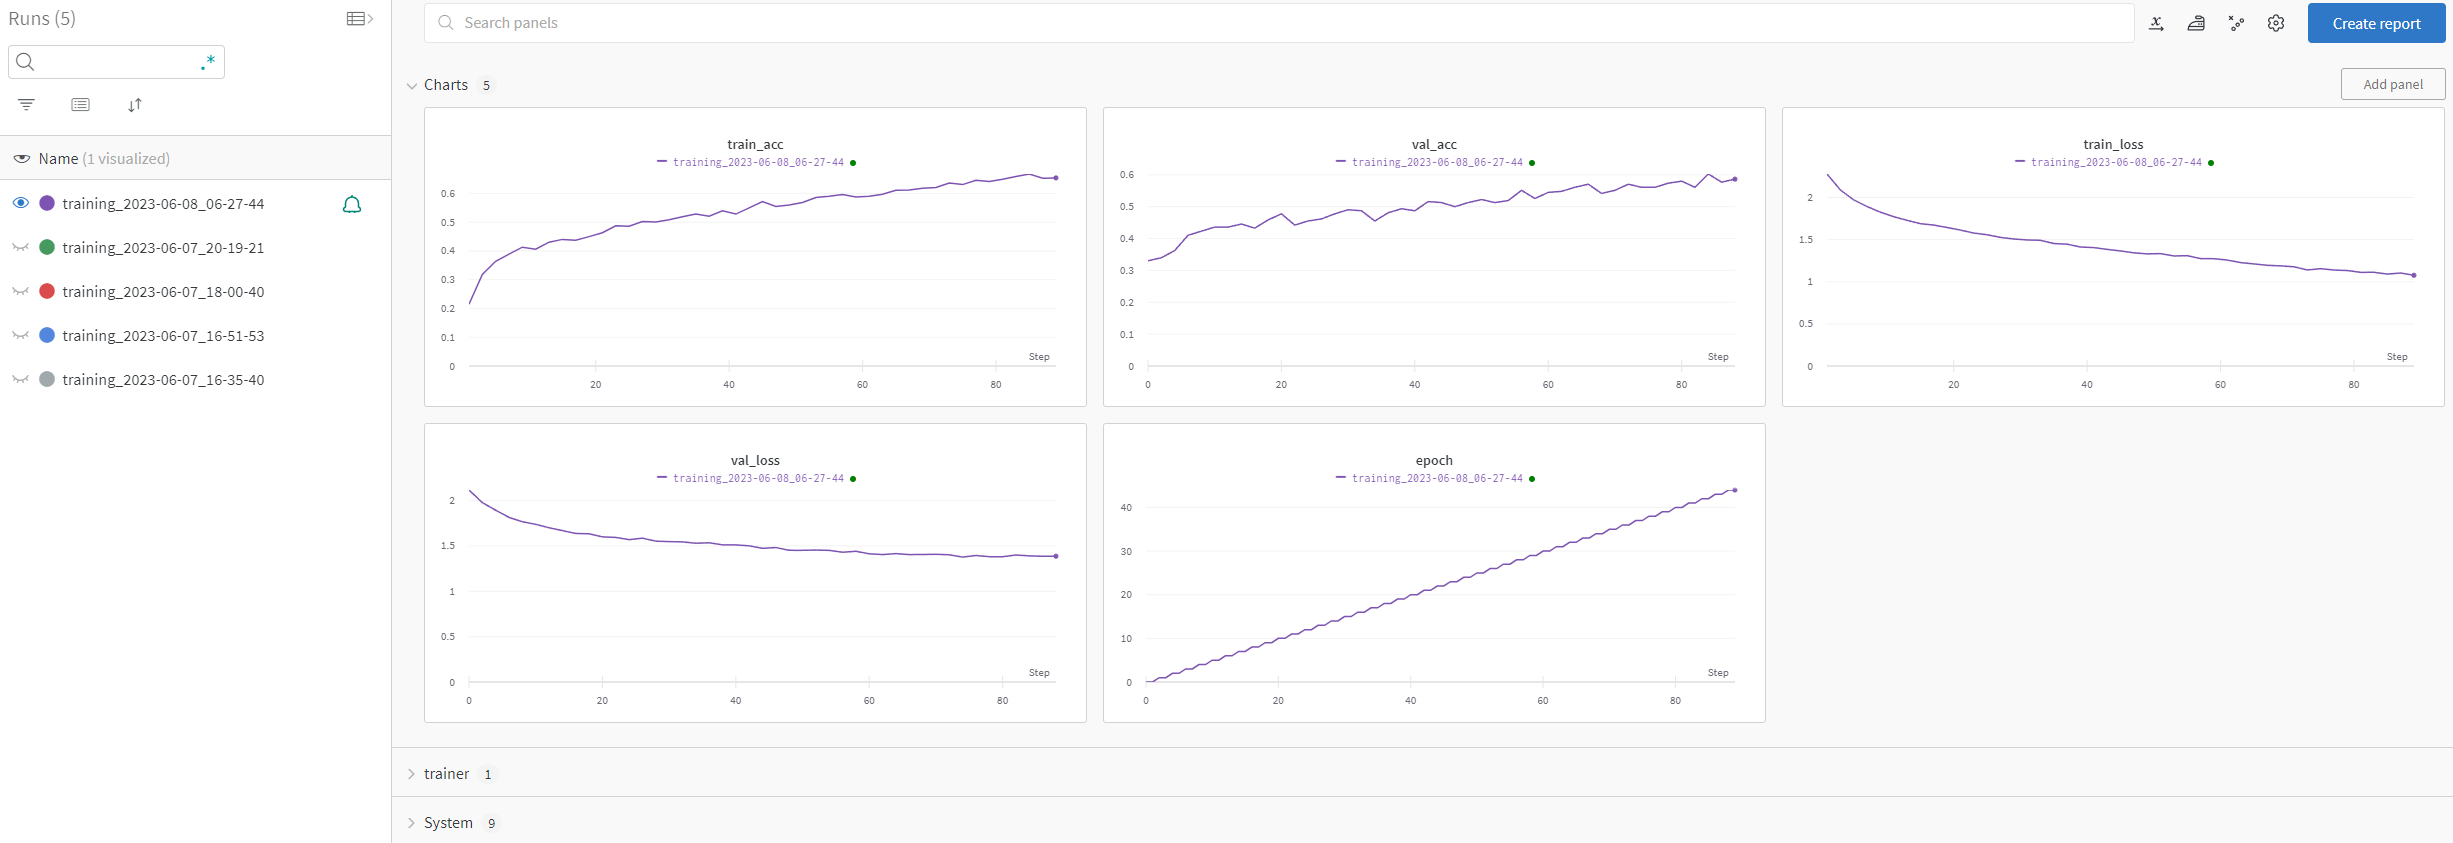
\includegraphics[width=\textwidth]{rsc/wandb_interface.png}
    \caption{Partie de l'interface de WandB montrant les métriques d'entraînement d'un modèle.}
    \label{fig:wandb}
\end{figure}

Nous utilisons également WandB pour régler les paramètres et hyper-paramètres liés à l'entraînement du modèle. En effet, il propose une fonctionnalité appelée \textit{Sweeps} qui permet de lancer plusieurs entraînements avec des paramètres différents et de visualiser les résultats obtenus. Le résultat de ce réglage est décrit dans la section \ref{sec:genre_detection}, relative au service intégrant le modèle de détection de style musical.

\subsection{Entraînement et déploiement automatique}\label{sec:train_deploy}

Le ré-entraînement et déploiement automatique d'un modèle de machine-learning est un objectif principal de ce projet intégré. Dans notre cas, le ré-entraînement du modèle est exécuté à travers une pipeline GitHub (\textit{GitHub Actions}) déclenchée à chaque push sur la branche develop de notre dépôt Git. Elle n'est pas déclenchée à chaque push sur la branche main afin qu'un dernier contrôle manuel puisse être effectué avant de déployer le modèle en production. La figure \ref{fig:training_pipeline} décrit le fonctionnement de cette pipeline.

\begin{figure}[H]
    \centering
    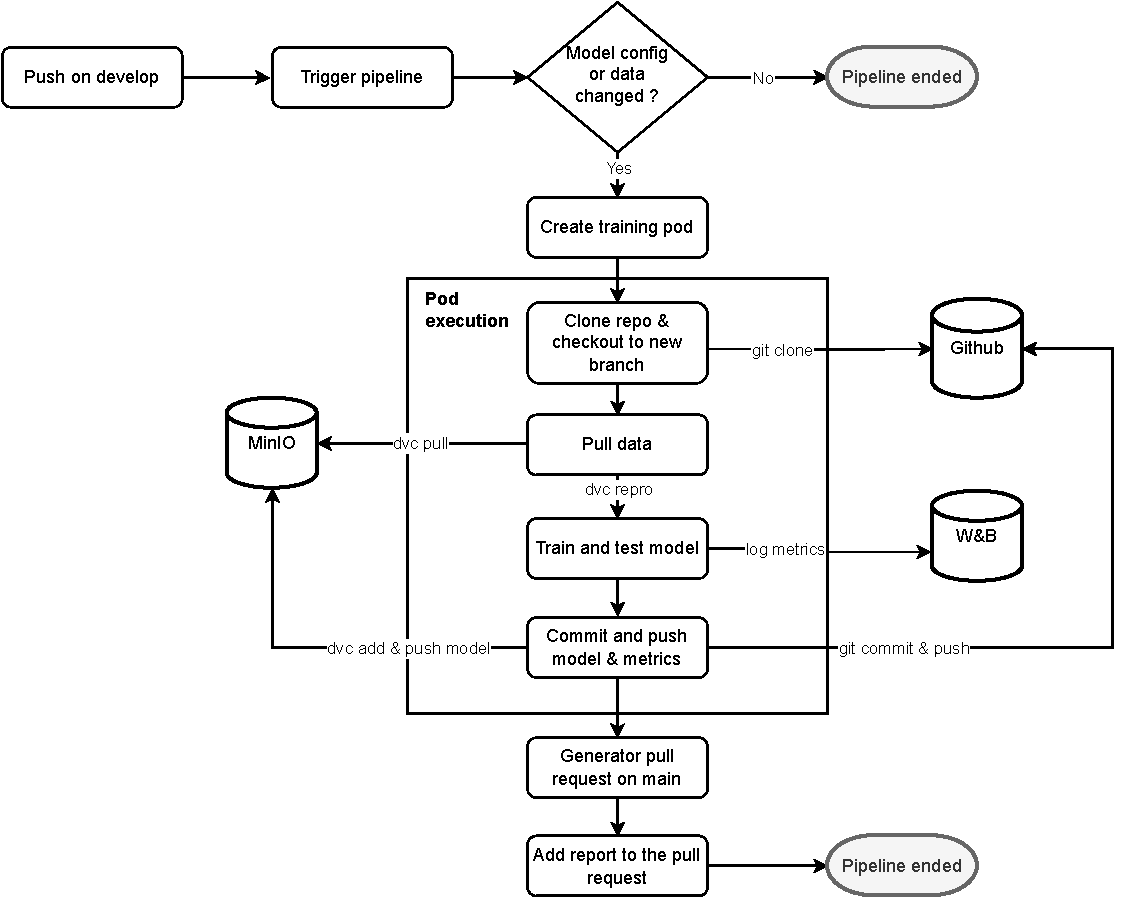
\includegraphics[width=0.68\textwidth]{rsc/training_pipeline.pdf}
    \caption{Pipeline d'entraînement du modèle de détection de genre musical.}
    \label{fig:training_pipeline}
\end{figure}

La pipeline vérifie, dans un premier temps, si les fichiers relatifs aux modèles (configuration, données, etc.) ont été modifiés. Si c'est le cas, elle lance l'exécution d'un job sur le cluster Kubernetes responsable de l'entraînement du modèle. De cette manière, nous pouvons avoir accès à des GPU si besoin et ne sommes pas dépendants des ressources des runners de GitHub. Dans l'exécution de ce job, le projet Git sur la branche develop est cloné, une nouvelle branche provisoire est créée et les données sont récupérées à l'aide de DVC. La commande \verb|dvc repro| permet de reproduire l'expérience d'entraînement et d'évaluation définie, au préalable, dans un fichier de configuration. Cette expérience comprend l'exécution du script d'entraînement du modèle (qui enregistre également les métriques d'entraînement vers WandB) ainsi que celui d'évaluation qui génère les métriques d'évaluation.

À la fin de l'expérience, les changements des fichiers trackés par DVC (modèles et métriques) sont enregistrés sur le serveur de stockage MinIO et tous les changements sont poussés vers le dépôt Git. Le job se termine et la pipeline GitHub génère une pull request sur la branche main, accompagnée d'un rapport comparant les métriques d'évaluation de l'expérience précédente aux nouvelles. En réalité, la génération de ce rapport d'utilisation est effectuée par une autre pipeline qui est déclenchée aussitôt qu'une pull request est créée sur la branche main. Le contenu de ce rapport dans la pull request est illustré à la figure \ref{fig:pull_request}.

\begin{figure}[H]
   \centering
   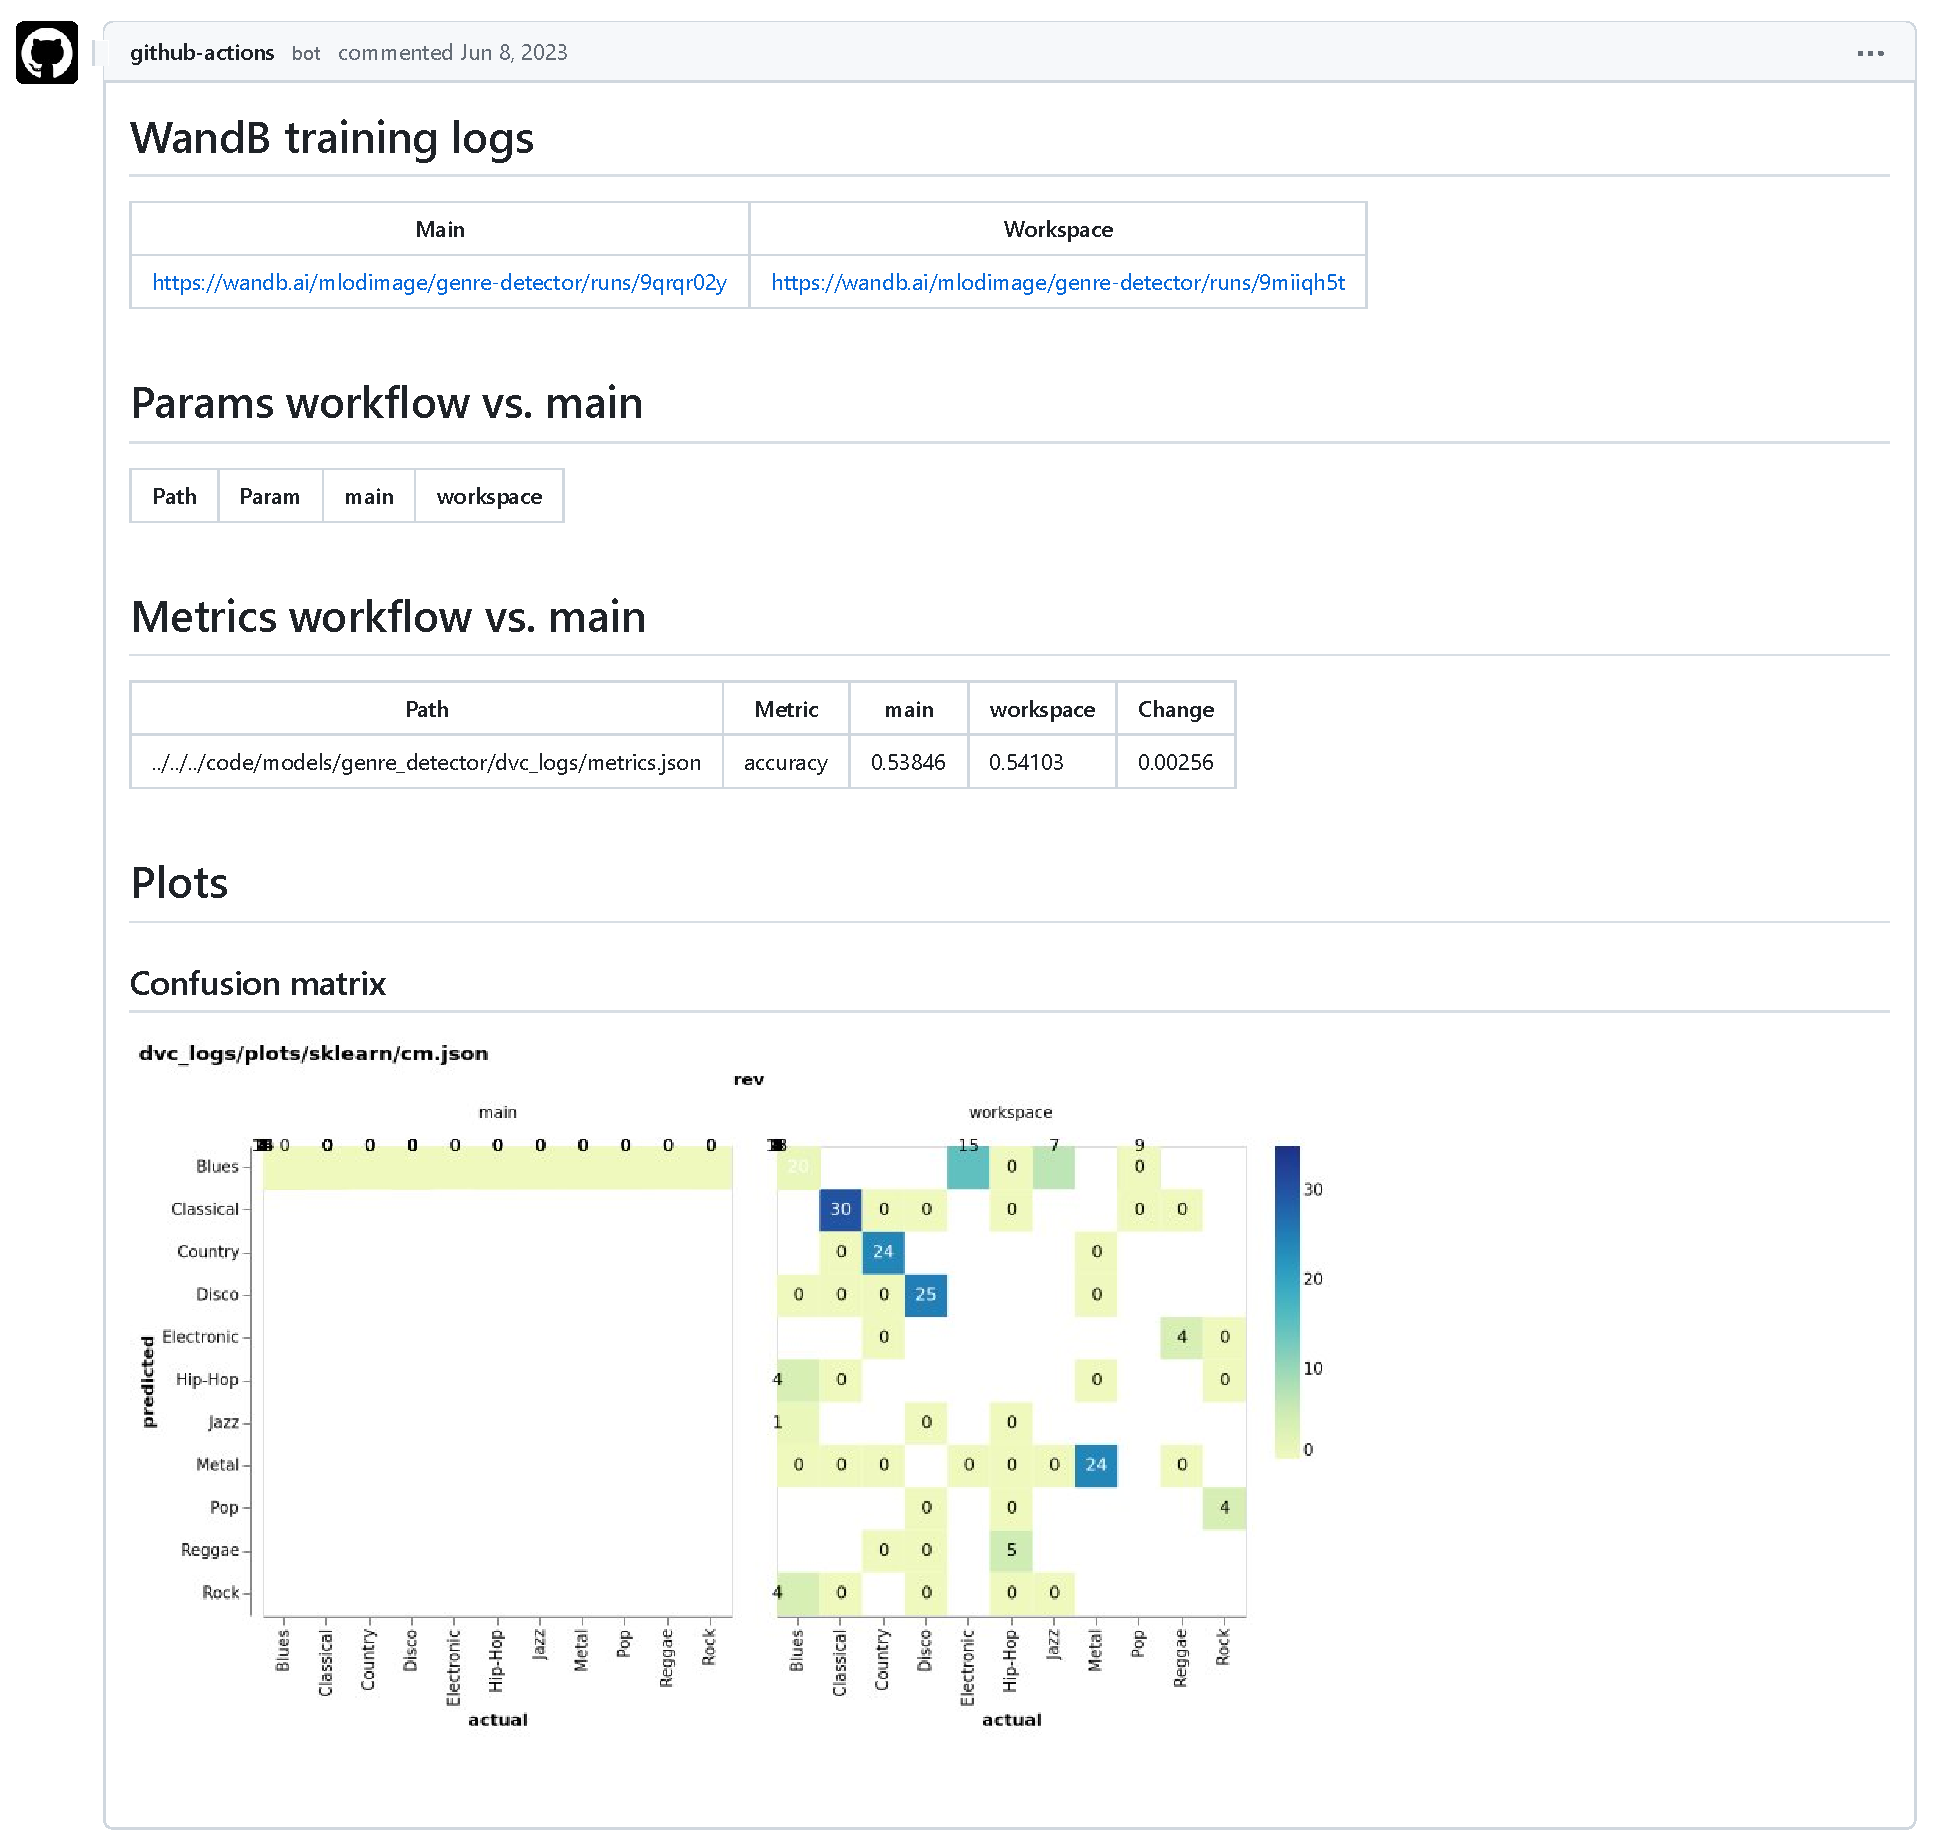
\includegraphics[width=0.8\textwidth]{rsc/report_pr.pdf}
   \caption{Contenu du rapport généré dans la pull request après l'entraînement d'un modèle.}
   \label{fig:pull_request}
\end{figure}

Ce rapport est généré à l'aide de l'outil CML, qui fait partie des outils proposés par l'entreprise Iterative AI, dont DVC fait également partie. Son intégration est donc facilitée et permet de générer des rapports facilement montrant la différence des paramètres et métriques gérées et créés par DVC. Les matrices de confusion ne s'affichent pas correctement et nous n'avons pas pu résoudre ce problème au moment de la rédaction de ce rapport. La figure \ref{fig:confusion_matrix} de la section \ref{subsec:training_results} montre une matrice de confusion générée correctement avant son intégration au rapport.

À noter que le Pod qui est exécuté dans le job Kubernetes d'entraînement se trouve dans le dossier service. C'est-à-dire qu'à chaque fois que ce dernier est modifié sur la branche main, la pipeline de déploiement va le considérer comme un service à déployer. L'image de ce Pod va donc être reconstruite, mais pas lancée en tant que service, grâce au fichier \verb|.build-only| qui indique de mettre à jour uniquement l'image sur la registry du projet.

